\begin{frame}{Traffic Analytics from a Fixed Camera}
  \begin{columns}[T,onlytextwidth]
    \column{0.55\textwidth}
      \begin{itemize}\footnotesize\itemsep0.3em
        \item \textbf{Pipeline:} counts, speeds and queues follow each vehicle across frames, so a detector (YOLO) is followed by a tracker that links boxes into identities. A homography $H$, a $3\times3$ matrix fitted from four or more road points with known map positions, maps the road plane in the image to metres.
        \item \textbf{Speed:} map the ground-contact point $p_t$ of a track (bottom centre of its box) with $H$, then $v \approx f\,\lVert H(p_t) - H(p_{t-k})\rVert / k$, with $f$ the frame rate and $k$ the frame gap. \textbf{Counts:} tracks that cross a virtual line or enter a polygon zone.
        \item \textbf{Across cameras:} re-identification matches a vehicle by appearance; a licence plate adds a near-unique key, which can be hashed on the camera when only the match is needed.
        \item \textbf{AI City Challenge 2024} (CVPR workshop): 726 teams from 47 countries and regions; tracks included traffic-safety video captioning and fisheye road-object detection.
      \end{itemize}
    \column{0.43\textwidth}
      \centering
      \vspace{0.2em}
      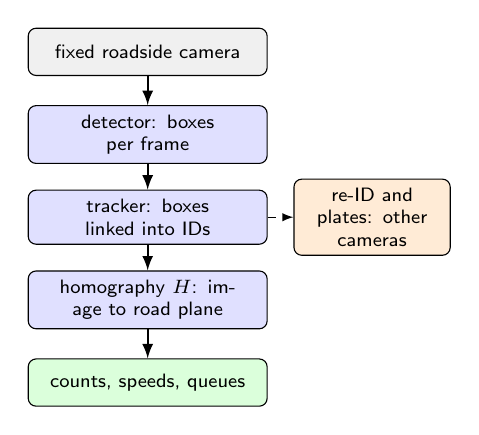
\begin{tikzpicture}[font=\sffamily\scriptsize, >=latex,
          box/.style={draw, rounded corners=0.1cm, align=center, text width=2.8cm, minimum height=0.6cm},
          src/.style={box, fill=gray!12},
          stage/.style={box, fill=blue!12},
          meas/.style={box, fill=green!14},
          sidebox/.style={box, fill=orange!16, text width=1.75cm}]
        \node[src] (cam) at (0,0) {fixed roadside camera};
        \node[stage] (det) at (0,-1.05) {detector: boxes per frame};
        \node[stage] (trk) at (0,-2.1) {tracker: boxes linked into IDs};
        \node[stage] (hom) at (0,-3.15) {homography $H$: image to road plane};
        \node[meas] (res) at (0,-4.2) {counts, speeds, queues};
        \node[sidebox] (reid) at (2.85,-2.1) {re-ID and plates: other cameras};
        \draw[->, thick] (cam) -- (det);
        \draw[->, thick] (det) -- (trk);
        \draw[->, thick] (trk) -- (hom);
        \draw[->, thick] (hom) -- (res);
        \draw[->, dashed] (trk) -- (reid);
      \end{tikzpicture}\\[0.4em]
      {\scriptsize Open tools: Ultralytics YOLO (AGPL-3.0) ships six trackers, ByteTrack and BoT-SORT among them; supervision (MIT) adds line and polygon zone counters.\par}
  \end{columns}
  \vspace{0.3em}
  {\scriptsize Wang et al., ``The 8th AI City Challenge,'' CVPR Workshops 2024, \href{https://arxiv.org/abs/2404.09432v1}{arXiv:2404.09432v1}; \href{https://docs.ultralytics.com/modes/track/}{docs.ultralytics.com/modes/track}; \href{https://github.com/roboflow/supervision}{github.com/roboflow/supervision}.\par}
\end{frame}

\begin{frame}{Tracking by Detection: Predict, Match, Update}
  \begin{columns}[T,onlytextwidth]
    \column{0.55\textwidth}
      \begin{itemize}\footnotesize\itemsep0.3em
        \item \textbf{SORT} (Simple Online and Realtime Tracking) keeps one \textbf{Kalman filter} per track: a recursive estimator for a linear motion model with Gaussian noise. It stores a mean state $\hat{x}$ and a covariance $P$, and runs two steps per frame:
        \[ \begin{aligned}
          \text{predict:}\quad & \hat{x}^- = F\hat{x}, \qquad P^- = FPF^\top + Q\\
          \text{gain:}\quad & K = P^-C^\top\,(CP^-C^\top + R)^{-1}\\
          \text{update:}\quad & \hat{x} = \hat{x}^- + K\,(z - C\hat{x}^-)\\
          & P = (I - KC)\,P^-
        \end{aligned} \]
        {\scriptsize $F$ adds each velocity to its position (constant-velocity model); $Q$ and $R$ are the motion and detection noise covariances; $C$ reads the box out of the state; $z$ is the matched detection. The gain $K$ leans towards whichever of prediction and detection is less uncertain.\par}
        \item SORT's state is $x = [u, v, s, r, \dot{u}, \dot{v}, \dot{s}]^\top$: box centre $(u, v)$, area $s$, aspect ratio $r$ (held constant), and three velocities.
      \end{itemize}
    \column{0.43\textwidth}
      {\centering
      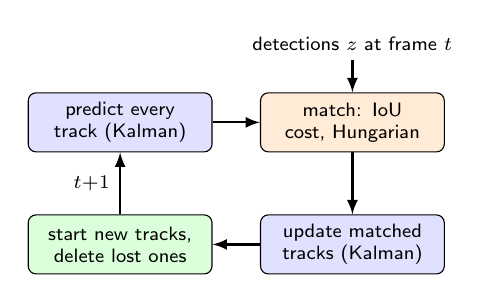
\begin{tikzpicture}[font=\sffamily\scriptsize, >=latex,
          stepbox/.style={draw, rounded corners=0.1cm, align=center, text width=2.1cm, minimum height=0.75cm},
          kal/.style={stepbox, fill=blue!12},
          asg/.style={stepbox, fill=orange!16},
          life/.style={stepbox, fill=green!14}]
        \node[kal] (pred) at (0,0) {predict every track (Kalman)};
        \node[asg] (match) at (2.95,0) {match: IoU cost, Hungarian};
        \node[kal] (upd) at (2.95,-1.55) {update matched tracks (Kalman)};
        \node[life] (bd) at (0,-1.55) {start new tracks, delete lost ones};
        \node (dets) at (2.95,1.0) {detections $z$ at frame $t$};
        \draw[->, thick] (dets) -- (match);
        \draw[->, thick] (pred) -- (match);
        \draw[->, thick] (match) -- (upd);
        \draw[->, thick] (upd) -- (bd);
        \draw[->, thick] (bd) -- node[left] {$t{+}1$} (pred);
      \end{tikzpicture}\par}
      \begin{itemize}\scriptsize\itemsep0.2em
        \item \textbf{Match:} an IoU-based cost between every predicted box and every detection, solved by the Hungarian algorithm (the lowest-cost one-to-one pairing, also used by DETR); pairs below a minimum IoU are rejected.
        \item \textbf{Birth and death:} unmatched detections open tentative tracks, confirmed by later matches; SORT deletes a track after one missed frame, since constant-velocity guesses drift fast.
        \item Tracking ran at 260\,Hz on one CPU core; detection quality was a key factor (a better detector improved tracking by up to 18.9\%).
      \end{itemize}
  \end{columns}
  \vspace{-0.6em}
  {\scriptsize Bewley et al., ``Simple Online and Realtime Tracking,'' ICIP 2016, \href{https://arxiv.org/abs/1602.00763v2}{arXiv:1602.00763v2}, abstract, Secs.~3--4.\par}
\end{frame}

\begin{frame}{ByteTrack: Keep the Low-Score Boxes}
  \begin{columns}[T,onlytextwidth]
    \column{0.40\textwidth}
      \centering
      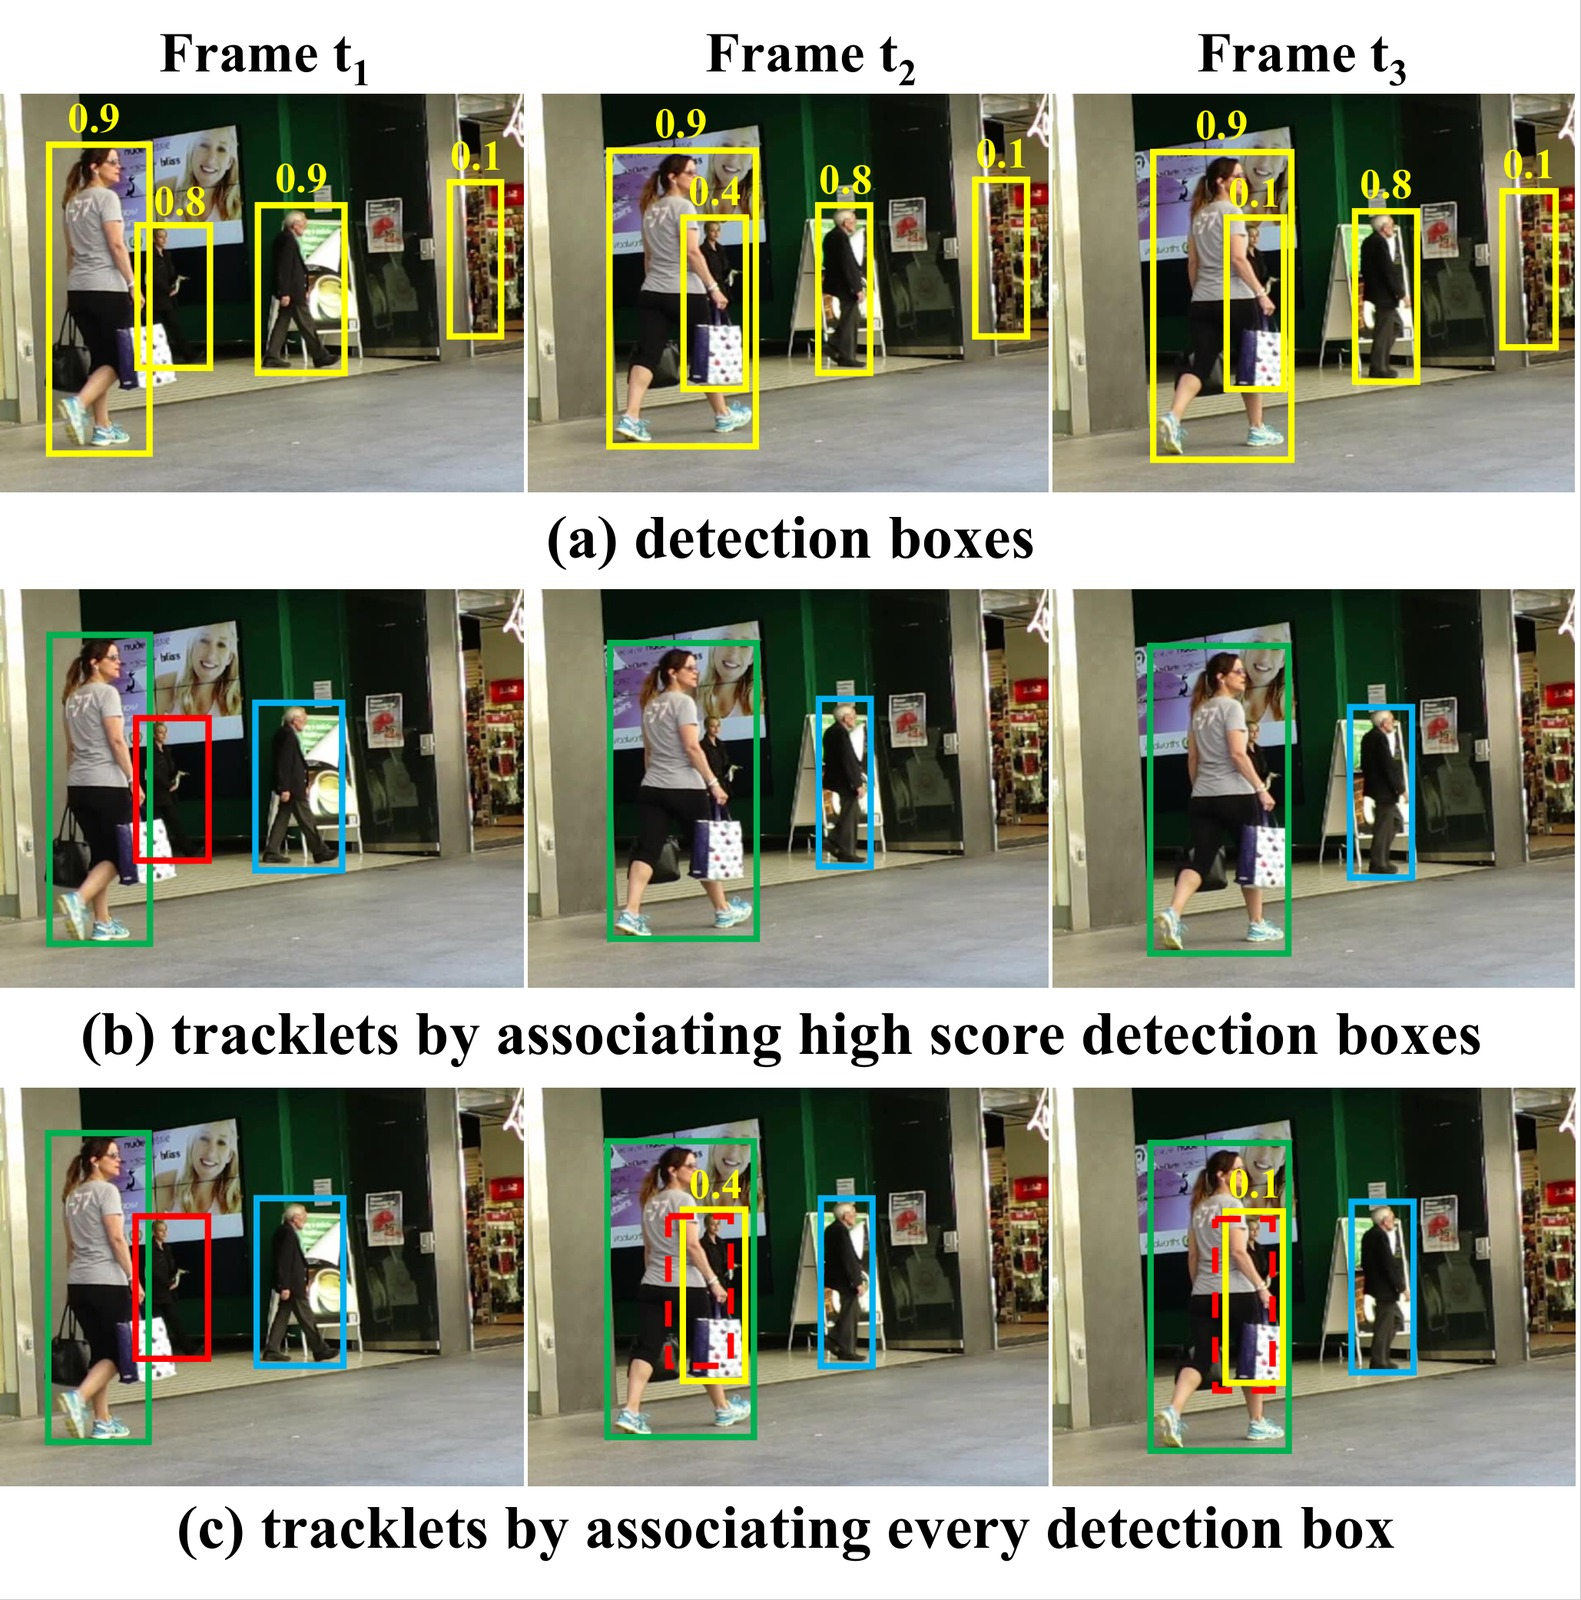
\includegraphics[width=\linewidth,height=0.66\textheight,keepaspectratio]{images/image-restoration-applications/bytetrack_fig2_low_score_association.jpg}\\[0.2em]
      {\scriptsize Zhang et al., ``ByteTrack: Multi-Object Tracking by Associating Every Detection Box,'' ECCV 2022, \href{https://arxiv.org/abs/2110.06864v3}{arXiv:2110.06864v3}, Figure~2.\par}
    \column{0.58\textwidth}
      \begin{itemize}\footnotesize\itemsep0.3em
        \item Occlusion lowers detection scores: the person walking behind the woman scores 0.8, 0.4, then 0.1. A fixed score threshold drops those boxes and the track breaks (b).
        \item \textbf{BYTE}, ByteTrack's matching step, splits detections at $\tau = 0.6$. High-score boxes are matched to all tracks first (IoU or re-ID cost); low-score boxes are then matched to the tracks still unmatched, by IoU only, since appearance fails under occlusion and blur. Leftover low-score boxes are discarded as background (c).
        \item On the MOT17 pedestrian validation set, BYTE in place of SORT's matching raises MOTA from 74.6 to 76.6 and IDF1 from 76.9 to 79.3, and cuts identity switches from 291 to 159. ByteTrack (a YOLOX detector plus BYTE) reaches 80.3 MOTA, 77.3 IDF1 and 63.1 HOTA on MOT17 test at 30 FPS on one V100.
      \end{itemize}
      \vspace{0.2em}
      {\scriptsize \textbf{Scores.} $\mathrm{MOTA} = 1 - (\mathrm{FN} + \mathrm{FP} + \mathrm{IDSW})/\mathrm{GT}$ charges misses, false alarms and identity switches per ground-truth box. $\mathrm{IDF1} = \mathrm{IDTP}/(\mathrm{IDTP} + \tfrac{1}{2}\mathrm{IDFN} + \tfrac{1}{2}\mathrm{IDFP})$ is the share of boxes that carry the right identity under one global matching of tracks to ground truth. $\mathrm{HOTA}$ averages $(\mathrm{DetA}_\alpha\cdot\mathrm{AssA}_\alpha)^{1/2}$, detection times association accuracy, over localisation thresholds $\alpha$ (Luiten et al., IJCV 2021, \href{https://arxiv.org/abs/2009.07736v2}{arXiv:2009.07736v2}).\par}
  \end{columns}
\end{frame}

\begin{frame}{Camera-Only Bird's-Eye-View Perception}
  \begin{columns}[T,onlytextwidth]
    \column{0.45\textwidth}
      \begin{itemize}\footnotesize\itemsep0.35em
        \item \textbf{Bird's-eye view (BEV):} a top-down grid around the car where detection, lane maps and planning share one frame. BEVFormer uses $200\times200$ cells of 0.512\,m.
        \item \textbf{Lift-Splat-Shoot (LSS):} each pixel predicts a context vector $c \in \mathbb{R}^C$ and a distribution $\alpha$ over depth bins $D$. The feature placed at depth $d$ on the pixel's ray is $c_d = \alpha_d\, c$; the camera's calibration (focal length, principal point, mounting pose) fixes where that 3D point lies around the car. Splat: sum-pool all points into vertical pillars, giving a $C$-channel BEV map for a CNN.
        \item \textbf{Occupancy} (Occ3D): a free or occupied label and a class for every voxel, so irregular shapes and object types missing from the label list are still represented.
      \end{itemize}
    \column{0.53\textwidth}
      {\centering
      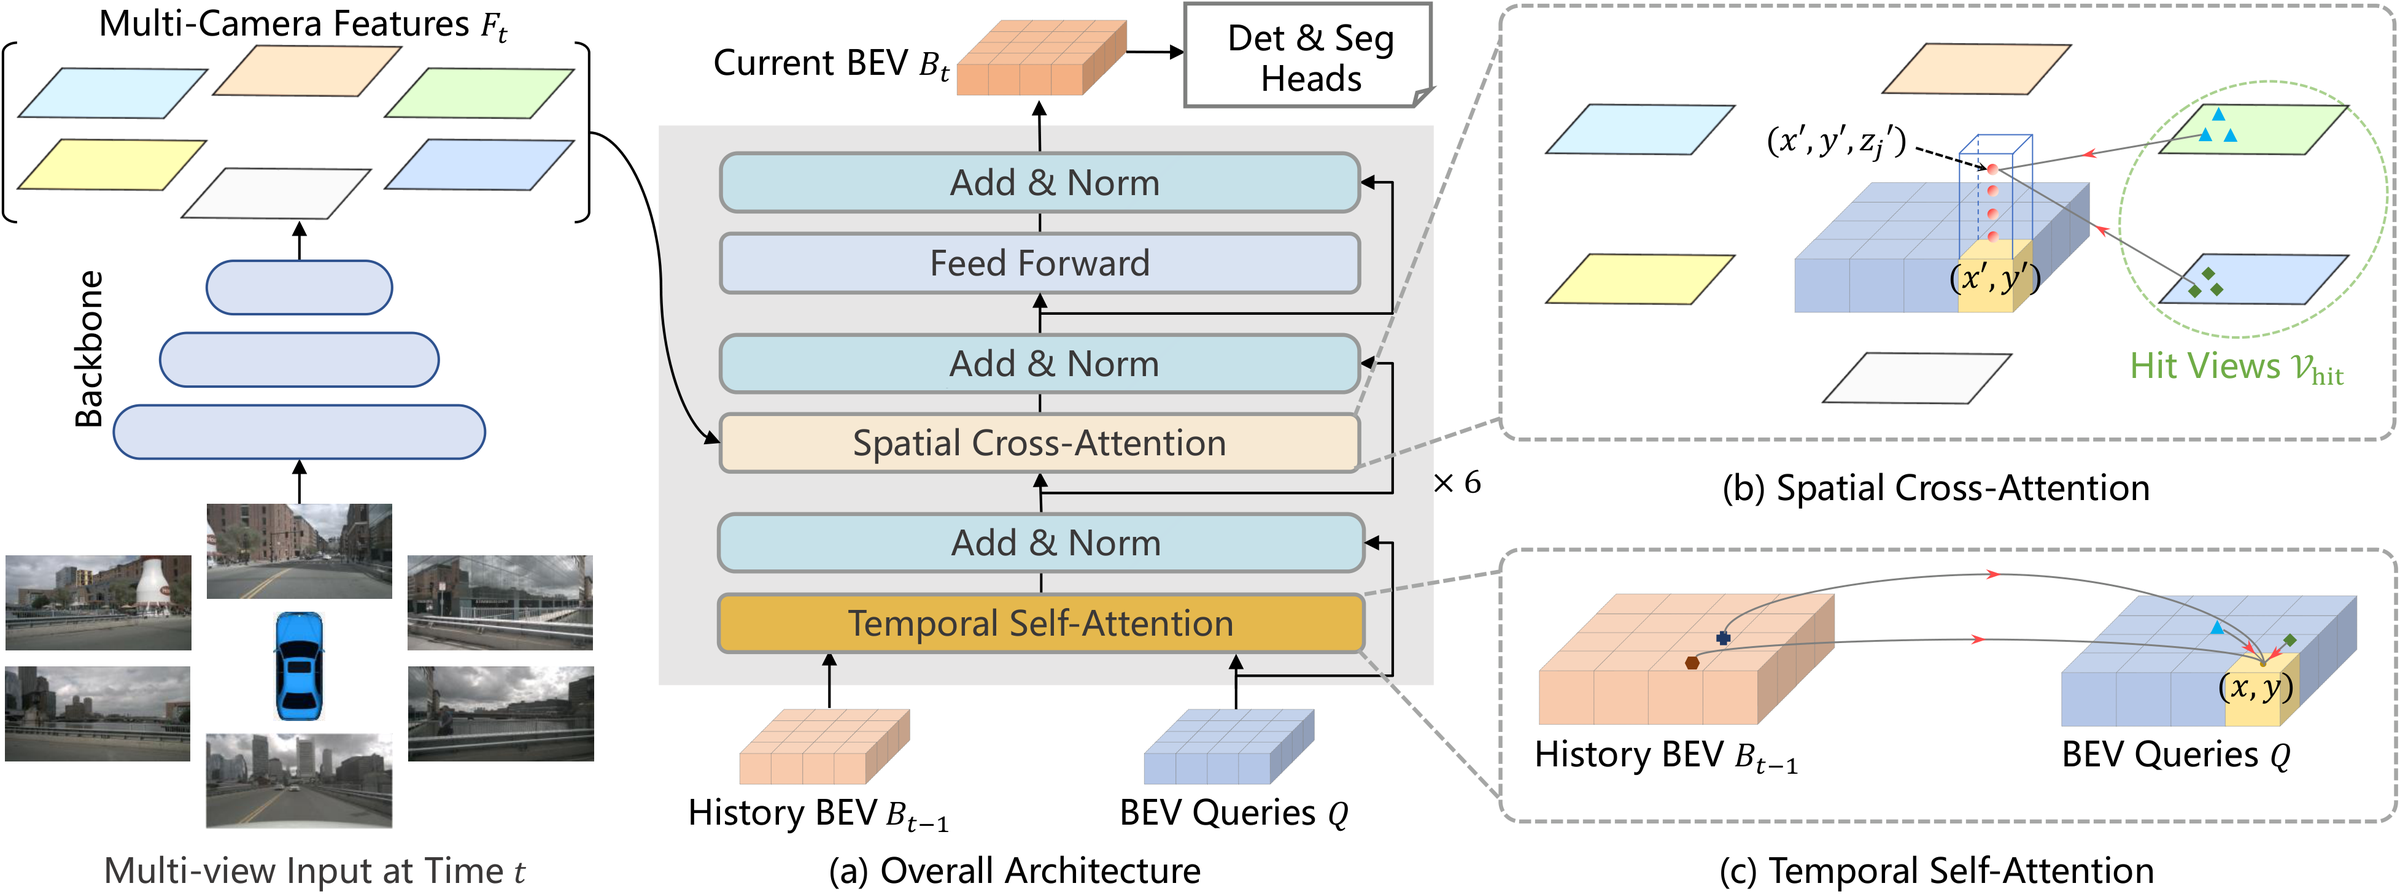
\includegraphics[width=\linewidth,height=0.33\textheight,keepaspectratio]{images/image-restoration-applications/bevformer_fig2_architecture.png}\\[0.2em]
      {\scriptsize Li et al., ``BEVFormer: Learning Bird's-Eye-View Representation from Multi-Camera Images via Spatiotemporal Transformers,'' ECCV 2022, \href{https://arxiv.org/abs/2203.17270v2}{arXiv:2203.17270v2}, Figure~2.\par}\par}
      \begin{itemize}\scriptsize\itemsep0.2em
        \item \textbf{BEVFormer:} a grid of learnable BEV queries pulls features in. Spatial cross-attention (b) projects 4 points stacked above each cell into the cameras that see them and samples features only near those points; temporal self-attention (c) reads the previous BEV map $B_{t-1}$.
        \item 56.9\% NDS on the test split of nuScenes, a six-camera driving benchmark, 9.0 points above the previous best, DETR3D. NDS (nuScenes detection score) combines mAP with translation, scale, orientation, velocity and attribute errors.
      \end{itemize}
  \end{columns}
  \vspace{0.2em}
  {\scriptsize Philion and Fidler, ECCV 2020, \href{https://arxiv.org/abs/2008.05711v1}{arXiv:2008.05711v1}, Section~3; Tian et al., NeurIPS 2023, \href{https://arxiv.org/abs/2304.14365v3}{arXiv:2304.14365v3}.\par}
\end{frame}

\begin{frame}{End-to-End Driving: Planning-Oriented UniAD}
  \centering
  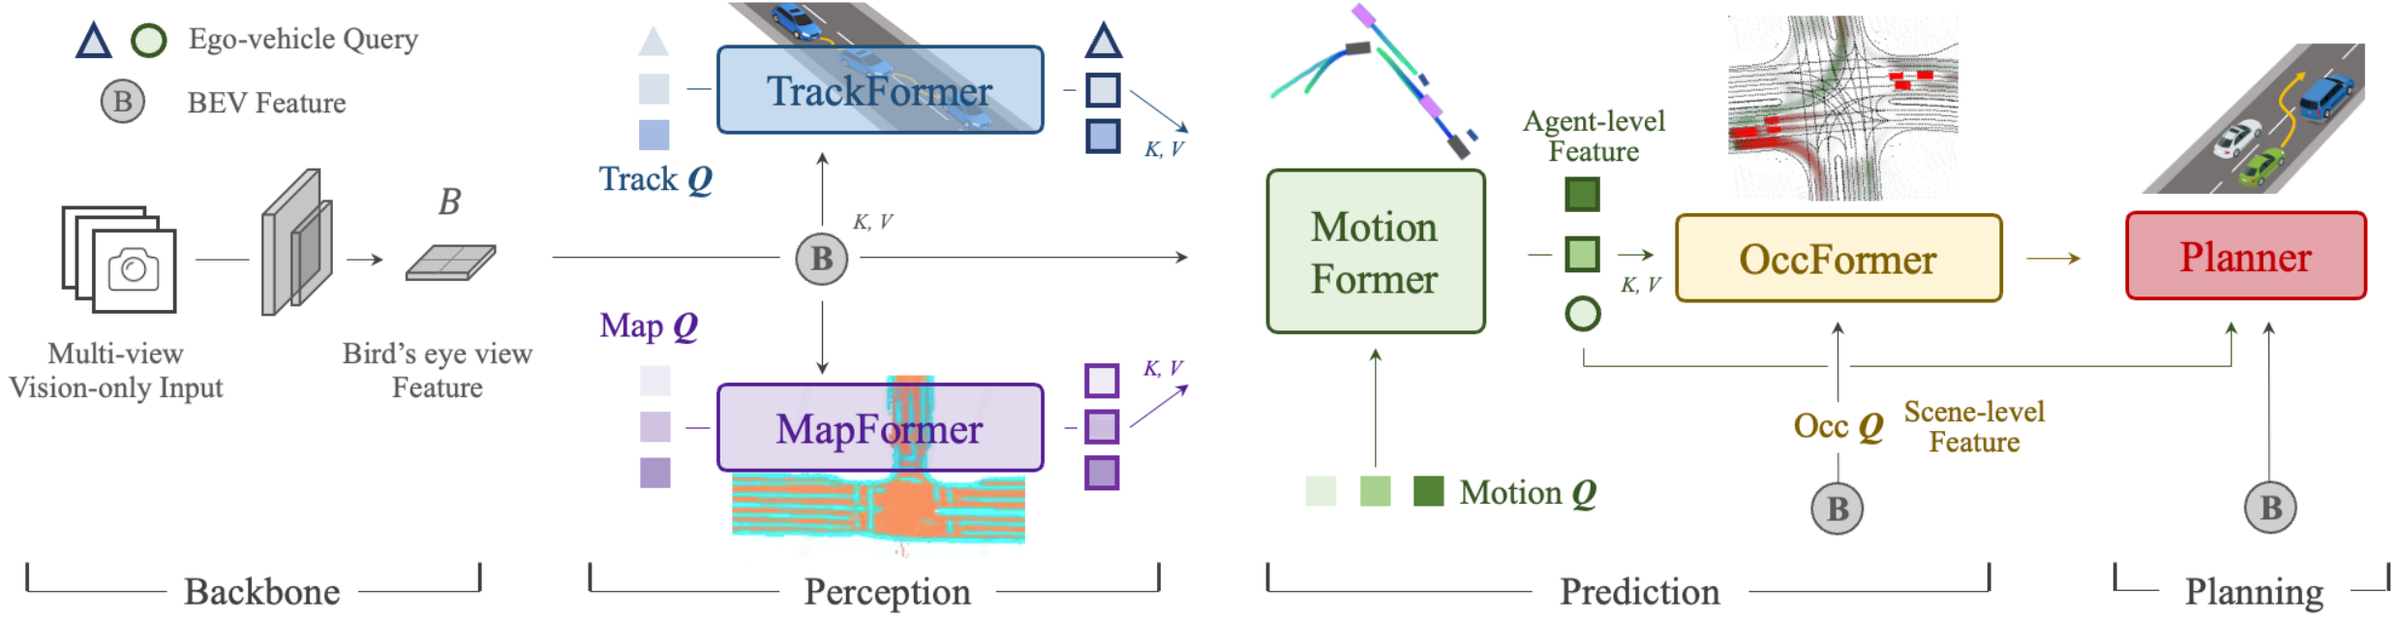
\includegraphics[width=\textwidth,height=0.34\textheight,keepaspectratio]{images/image-restoration-applications/uniad_fig2_pipeline.png}\\[0.2em]
  {\scriptsize Hu et al., ``Planning-oriented Autonomous Driving,'' CVPR 2023, \href{https://arxiv.org/abs/2212.10156v2}{arXiv:2212.10156v2}, Figure~2. Award: \href{https://www.computer.org/press-room/cvpr2023-best-paper-winners}{IEEE Computer Society, 21 June 2023}.\par}
  \vspace{0.3em}
  \begin{itemize}\footnotesize\itemsep0.3em
    \item A modular stack hands boxes and lanes from perception to prediction to planning through fixed interfaces, which risks information loss and error accumulation between modules.
    \item \textbf{UniAD} (Unified Autonomous Driving; CVPR~2023 Best Paper) keeps the modules but trains them as one network aimed at planning. BEV features come from the BEVFormer encoder; TrackFormer and MapFormer (perception) and MotionFormer and OccFormer (prediction) are transformer decoders that hand learned queries to the next stage; an ego-vehicle query carries the result to the planner.
    \item Reported nuScenes planning: L2 error 1.03\,m and collision rate 0.31\%, averaged over 1, 2 and 3\,s, the best in its comparison (Table~7). Both are open-loop metrics, computed against logged human driving.
  \end{itemize}
\end{frame}

\begin{frame}{Why Open-Loop Driving Scores Mislead}
  \begin{columns}[T,onlytextwidth]
    \column{0.50\textwidth}
      \begin{itemize}\footnotesize\itemsep0.3em
        \item \textbf{Open loop} replays a log and scores the plan against the human trajectory (L2 error, collisions); the plan never changes the scene. \textbf{Closed loop} lets the policy drive in a simulator.
        \item 73.9\% of nuScenes is near-straight driving. With no camera at all, an MLP on ego velocity, acceleration, yaw and driving command matches UniAD and VAD (another end-to-end planner) on L2 and collisions; its curb-collision rate is what separates it from UniAD.
      \end{itemize}
      \vspace{0.2em}
      {\centering\scriptsize
      \begin{tabular}{@{}l c c c@{}}
        \toprule
        nuScenes, 1--3\,s average & L2 (m) & Coll.\ (\%) & Curb (\%) \\
        \midrule
        UniAD (official) & 0.66 & 0.62 & 1.72 \\
        VAD-Base (official) & 0.37 & 0.33 & 2.47 \\
        Go straight, current speed & 0.83 & 1.08 & 8.62 \\
        Ego-MLP, no camera & 0.35 & 0.37 & 2.93 \\
        \bottomrule
      \end{tabular}\par}
      \vspace{0.2em}
      {\scriptsize Released checkpoints, rescored with corrected collision checks; the official UniAD checkpoint already feeds ego status into its BEV encoder, so its L2 beats the 1.03\,m its paper reported. Li et al., ``Is Ego Status All You Need for Open-Loop End-to-End Autonomous Driving?,'' CVPR 2024, \href{https://arxiv.org/abs/2312.03031v2}{arXiv:2312.03031v2}, Table~1 and Appendix~B.\par}
    \column{0.48\textwidth}
      {\centering
      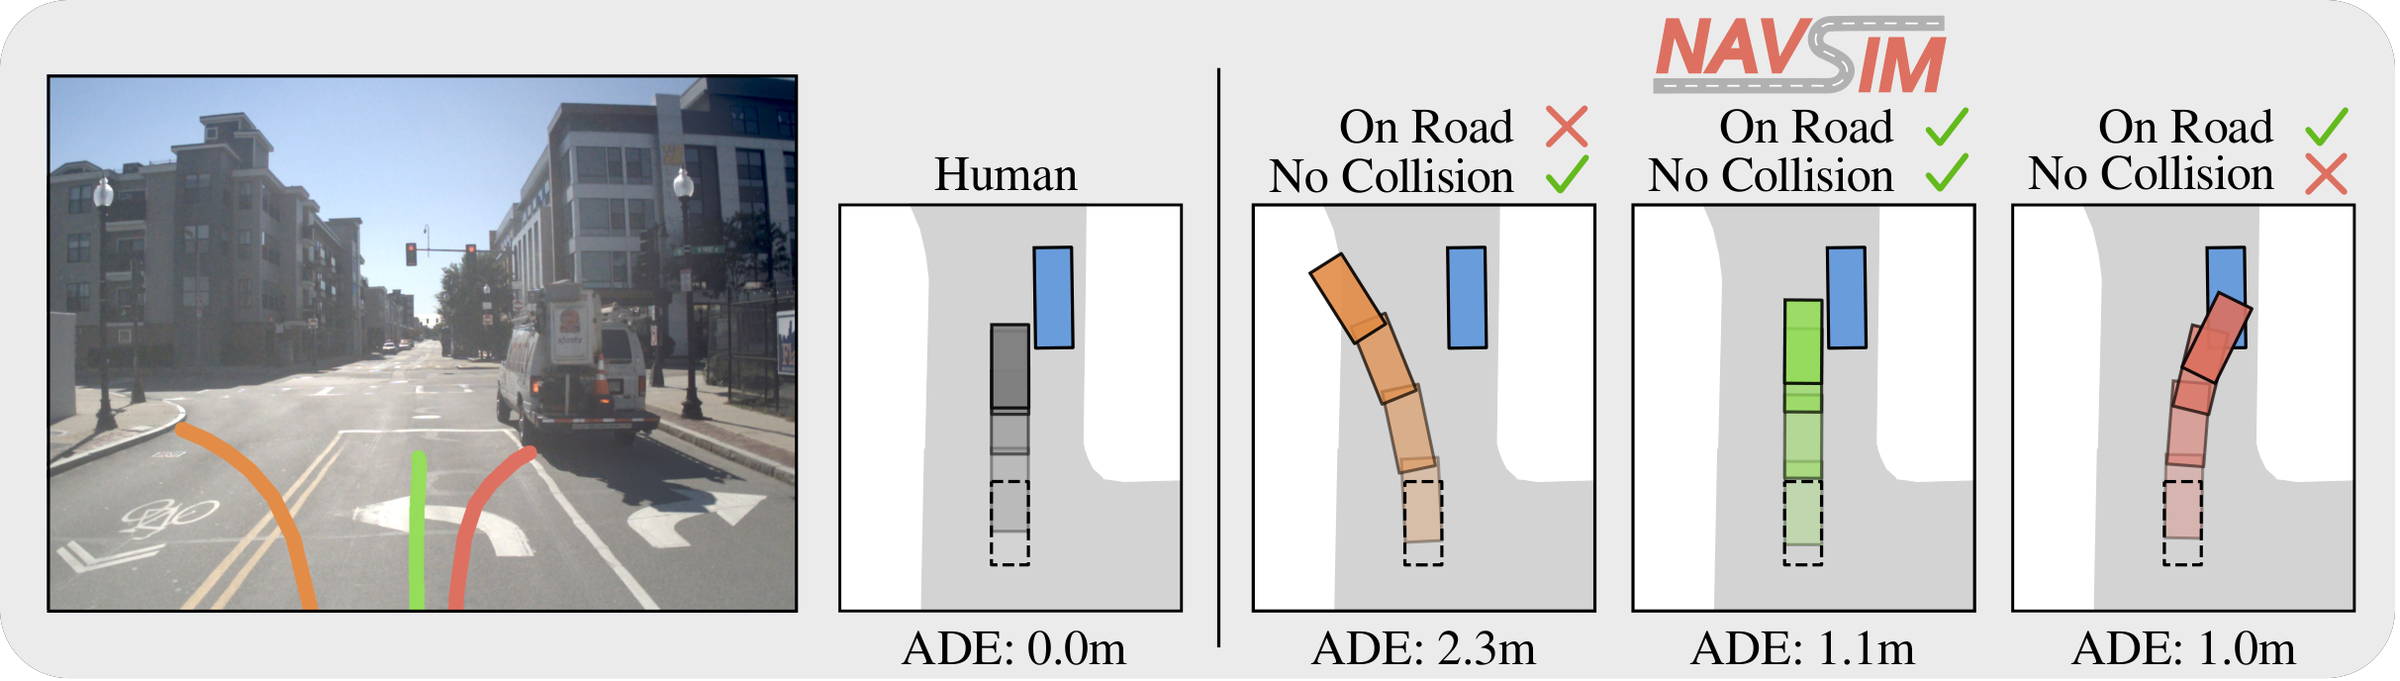
\includegraphics[width=\linewidth,height=0.24\textheight,keepaspectratio]{images/image-restoration-applications/navsim_fig1_ade_vs_safety.png}\\[0.1em]
      {\scriptsize Dauner et al., ``NAVSIM: Data-Driven Non-Reactive Autonomous Vehicle Simulation and Benchmarking,'' NeurIPS 2024, \href{https://arxiv.org/abs/2406.15349v2}{arXiv:2406.15349v2}, Figure~1.\par}\par}
      \begin{itemize}\scriptsize\itemsep0.2em
        \item \textbf{NAVSIM} rolls each test scene forward 4\,s without letting other agents react, then scores the plan with $\mathrm{PDMS} = \mathrm{NC}\cdot\mathrm{DAC}\cdot(5\,\mathrm{EP} + 5\,\mathrm{TTC} + 2\,\mathrm{C})/12$: no at-fault collision, drivable-area compliance, ego progress, time-to-collision margin, comfort. Scenes that constant velocity already solves are filtered out; there an ego-status MLP scores 65.6, UniAD 83.4, the human log 94.8.
        \item \textbf{Bench2Drive} runs closed loop in the CARLA simulator: 44 interactive scenarios (cut-ins, overtaking, detours) over 220 routes in varied towns and weathers; its training data span 23 weathers and 12 towns.
      \end{itemize}
  \end{columns}
\end{frame}

\begin{frame}{Driving Policies Since 2025: Diffusion and VLA}
  \footnotesize A \textbf{vision-language-action (VLA)} model is a vision-language model that also outputs actions.\par
  \vspace{0.1em}
  {\centering\scriptsize
  \begin{tabular}{>{\raggedright\arraybackslash}p{1.9cm} >{\raggedright\arraybackslash}p{5.5cm} >{\raggedright\arraybackslash}p{4.9cm}}
    \toprule
    \textbf{Model} & \textbf{How it plans} & \textbf{Reported result} \\
    \midrule
    DiffusionDrive (CVPR 2025) & denoises 20 $k$-means anchor trajectories, lightly noised, in 2 steps (a vanilla diffusion policy used 20), then scores them & 88.1 PDMS on NAVSIM navtest (camera and LiDAR); 45 FPS on an NVIDIA 4090 \\
    \addlinespace[0.2em]
    EMMA (Waymo, TMLR 2025) & Gemini-based multimodal LLM; instructions, ego state, trajectories and 3D locations all written as text & state-of-the-art open-loop planning on nuScenes; no LiDAR or radar, at most 4 camera frames \\
    \addlinespace[0.2em]
    Alpamayo-R1 (NVIDIA, 2025) & the Cosmos-Reason VLM writes a chain-of-causation explanation, a diffusion decoder emits the trajectory; supervised fine-tuning, then reinforcement learning & up to 12\% better planning on hard cases than a trajectory-only baseline; 35\% fewer close encounters in closed-loop simulation; 99\,ms latency \\
    \bottomrule
  \end{tabular}\par}
  \vspace{0.1em}
  \begin{itemize}\footnotesize\itemsep0.2em
    \item \textbf{Night:} the gap between camera-only LSS and a LiDAR-based PointPillars model widens at night (car IoU about 0.31 against 0.45); restoration before perception is one remedy to test, judged by the driving score.
    \item \textbf{Open weights:} Alpamayo-R1 (8.2B + 2.3B parameters; weights under the OpenMDW-1.1 licence) needs a GPU with 24\,GB or more; openpilot (MIT) upgrades driver assistance on 300+ supported cars.
  \end{itemize}
  \vspace{0.1em}
  {\scriptsize Liao et al., \href{https://arxiv.org/abs/2411.15139v3}{arXiv:2411.15139v3}, Tables~1--2; Hwang et al., \href{https://arxiv.org/abs/2410.23262v3}{arXiv:2410.23262v3}; NVIDIA, \href{https://arxiv.org/abs/2511.00088v2}{arXiv:2511.00088v2}; Philion and Fidler, Sec.~5.5; \href{https://huggingface.co/nvidia/Alpamayo-R1-10B}{Alpamayo-R1 model card}; \href{https://github.com/commaai/openpilot}{openpilot repository}.\par}
\end{frame}
